In this section, we describe the AR.Drone simulation model, which includes a sensor and motion model.
Furthermore, we describe how a visual map of the indoor environment can be made and how this map can be used by the AR.Drone to localize itself.

	\section{Pose estimation}
In order to initialize a visual localization and mapping algorithm, a good estimate of the position based on the internal sensors of the AR.Drone is essential. The AR.Drone has several sources of information available about its movements and the majority of its computing power is dedicated to combine these sources into combined estimates. Here this information is combined into a state vector, with all information needed to initialize visual localization and mapping.

The AR.Drone is equipped with a number of sensors, which give frequent updates about the motion. 
The inertial sensor measures the body accelerations and angular velocities.
A proprietary filter on board of the AR.Drone converts the angular velocities to an estimated attitude (orientation).
A sonar sensor is used to measure the altitude of the vehicle.
In addition to the body accelerations, the AR.Drone sends an estimate of its estimated body velocity.
This estimate is based on the inertia measurements and optical flow obtained from the relative motion between camera frames.
%Unfortunately, the details of this velocity estimation are
%currently
%not documented by the manufacturer.
The details of this algorithm are proprietary information of the manufacturer. 

The information from the sensors are used in an Extended Kalman Filter (EKF) to estimate the current position.
The EKF has been considered~\cite{julier2004unscented} the facto standard in the theory of nonlinear state estimation.
Our EKF state vector comprises a position vector $p^{W}$, velocity vector $v^{W}$, acceleration vector $a^{W}$ and attitude (orientation) vector $q^{W}$.
All vectors are 3-dimensional Cartesian coordinates.

\begin{equation}
x = [ p^{W}  v^{W}  a^{W}  q^{W} ]
\label{eq:EKF_state_vecor}
\end{equation}

The filtered attitude (orientation) from the proprietary onboard filter is written directly to the attitude vector $q^{W}$ of the state.
%This is possible because 
Steder et al. \cite{steder2008visual} found that roll and pitch measurements are accurate, even for low-cost sensors and can be directly integrated into the state.
The body accelerations can be used to estimate the current velocity of the vehicle.
%However, from experiments \ref{Section sec:exp_accel} we found that the low-cost acceleration sensor from the AR.Drone provides unreliable data.
However, we found that the low-cost acceleration sensor from the AR.Drone provides unreliable data.
This is modeled by a large uncertainty in the covariance matrix $Q$ of the EKF.

Unlike the acceleration data, the velocity estimate sent by the AR.Drone is accurate enough for integration into the state.
Based on the previous position $p_{t-1}$, the state's velocity $v_{t}$ and time between measurements, the new position $p_{t}$ can be calculated as follows:

\begin{equation}
p_{t} = p_{t-1} + v_{t} \times \Delta t + a_{t} \times 0.5 \Delta t^2
\end{equation}
where $\Delta t$ is the variable time (seconds) between the last two measurements.
The body accelerations or velocity is sufficient to estimate the vehicle's altitude.
However, the sonar's altitude measurement can be integrated into the EKF to improve the altitude estimate.
The sonar sensor is not sensitive to drift because it provides an absolute altitude measurement.
Relying only on the sonar sensor is not optimal since the measurements depend heavily on material and structure of the floor.


		\subsection{Inertia measurements}
		\subsection{Onboard filtered measurements}
		\subsection{Vision-based velocity}
	\section{Mapping}
		\subsection{Visual map}

Now that we have an estimate of the AR.Drone's position and attitude in the world, we can use this information to build a visual map of the environment.
The AR.Drone is equipped with a down-looking camera that has a resolution of $176 \times 144$ pixels.
The frames captured by this camera can be warped on a flat canvas to create a visual map.
Directly merging the frames on the canvas is not possible, because individual frames can be taken from a broad range of angles and altitudes.
Instead, perspective correction is applied and all frames are normalized in size and orientation.

Before describing how a frame is warped, some basics about image formation are explained. %the camera matrix are explained.
The AR.Drone's camera is modeled using a pinhole camera model (Figure \ref{fig:mapping1}).
In this model, a scene view is formed by projecting 3D points into the image plane using a perspective transformation.
3D camera coordinates are typically described with homogeneous coordinates.

\begin{figure}[htb]
\centering
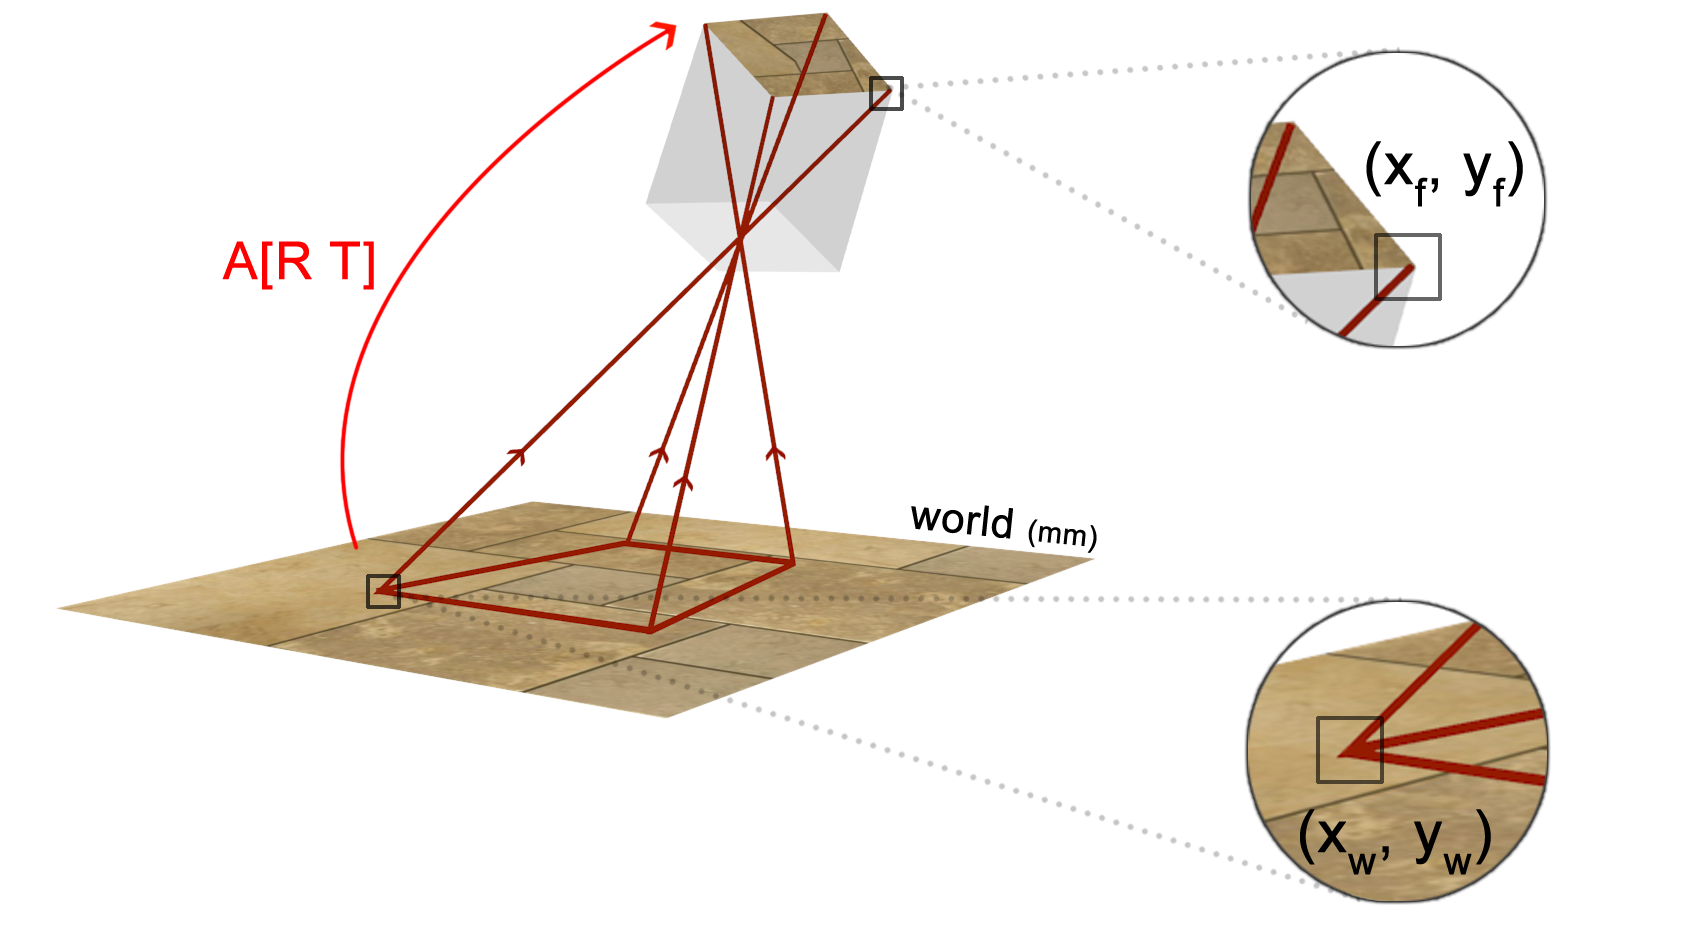
\includegraphics[width=10cm]{images/mapping0.png}
\caption{In the pinhole camera model, a scene view is formed by projecting 3D points into the image plane using a perspective transformation.}
\label{fig:mapping1}
\end{figure}

\begin{equation}
\left[ {
\begin{array}{c} x_f \\ y_f \\ 1 \end{array}
} \right]
= A[R|t]
\left[ {
\begin{array}{c} x_w \\ y_w \\ z_w \\ 1 \end{array}
} \right]
\end{equation}
where $x_f$ and $y_f$ represent a 2D point in pixel coordinates and $x_w$, $y_w$ and $z_w$ represent a 3D point in world coordinates.
The $3 \times 3$ \textit{camera intrinsic} matrix $A$ includes the camera's focal length and principal point.
The $3 \times 4$ joint rotation-translation matrix $[R|t]$ includes the \textit{camera extrinsic} parameters, which denote the coordinate system transformations from 3D world coordinates to 3D camera coordinates. Equivalently, the extrinsic parameters define the position of the camera center and the camera's heading (attitude) in world coordinates.

\begin{figure}[htb]
\centering
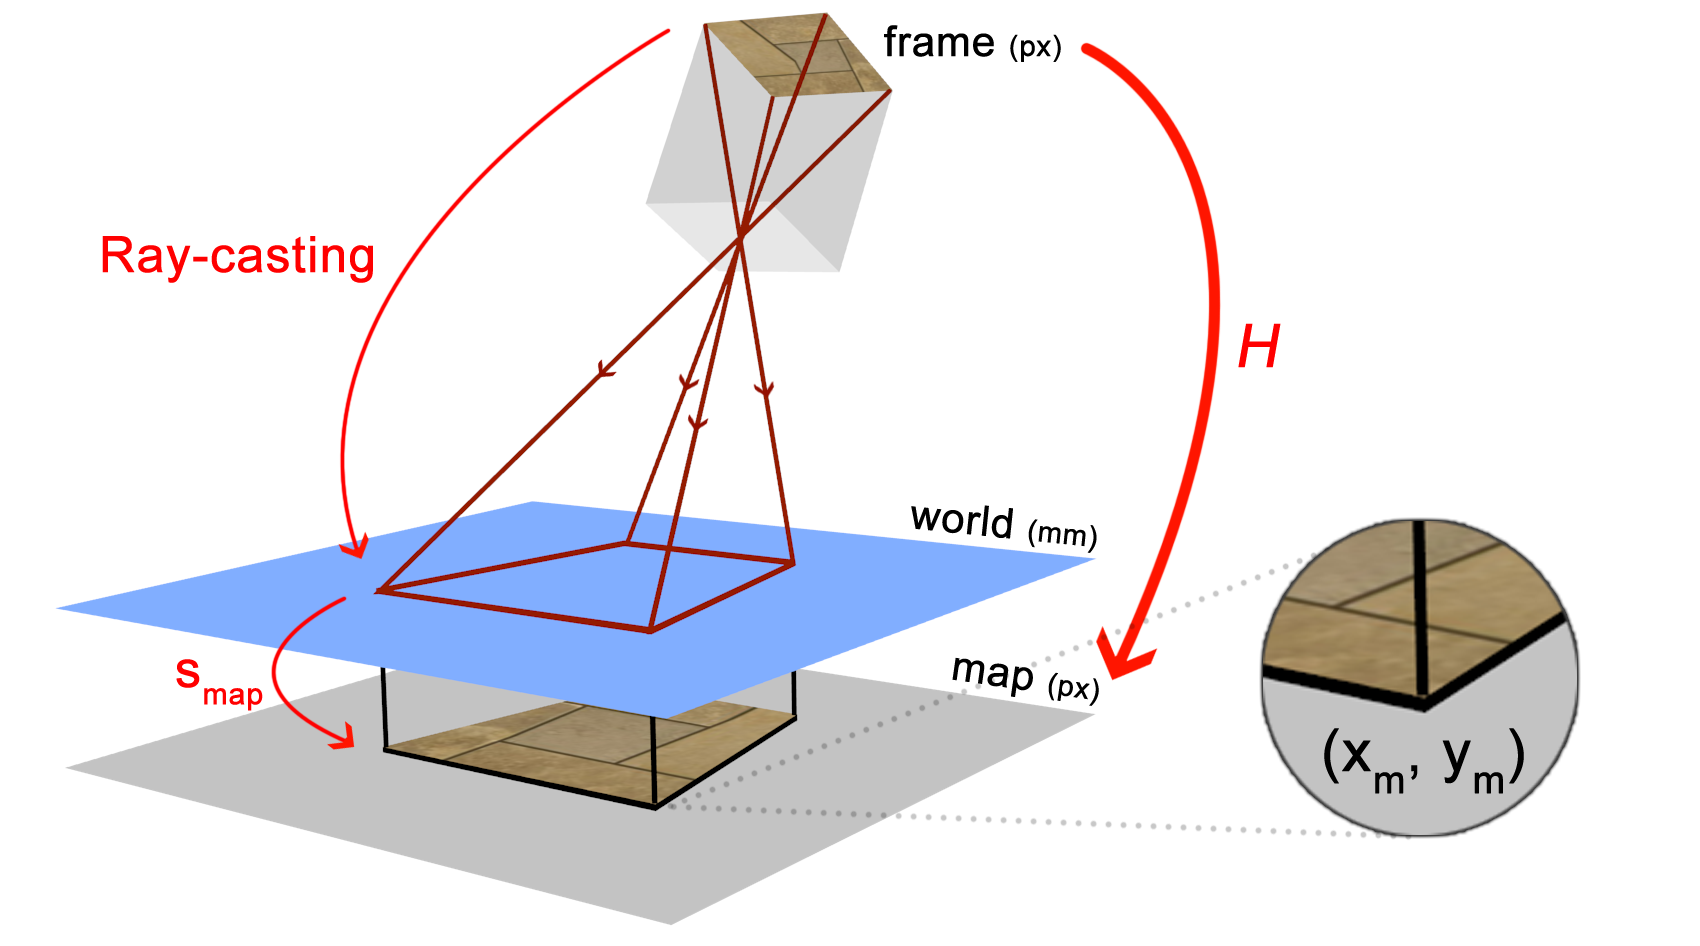
\includegraphics[width=10cm]{images/mapping1.png}
\caption{Visual map: warping a camera frame on the map's canvas. The frame's corners ($\small{px}$) are mapped to 2D world coordinates that lie on the world's plane. The 2D world coordinates of the frame are mapped to the map's canvas coordinates ($\small{px}$).}
\label{fig:mapping2}
\end{figure}

In order to warp a camera frame on the correct position of the canvas, we need to know which area of the world (floor) is captured by the camera.
This is the inverse operation of the image formation described above.
Instead of mapping 3D world coordinates to 2D pixel coordinates, 2D pixel coordinates are mapped to 3D world coordinates ($\small{mm}$).
It is impossible to recover the exact 3D world coordinates, because a pixel coordinate maps to a line instead of a point (i.e., multiple points in 3D world coordinates map to the same 2D pixel coordinate).
\begin{comment}
This is represented in the scaling factor $s$ in the next equation:

\begin{equation}
s \cdot \left[ {
\begin{array}{c} x_w \\ y_w \\ z_w \\ 1 \end{array}
} \right]
= A^{-1}[R|t]
\left[ {
\begin{array}{c} x_f \\ y_f \\ 1 \end{array}
} \right]
\end{equation}
\end{comment}
This ambiguity can be resolved by assuming that all 3D world points lie on a plane ($z_w = 0$), which makes it possible to recover $x_w$ and $y_w$.
The 2D world coordinates of the frame's corners are obtained by casting rays from the four frame's corners (top of Figure \ref{fig:mapping2}).
The 2D world coordinate that corresponds to a frame corner is defined as the point $(x_w,  y_w , 0)$ where the ray intersects the world plane ($z_w = 0$).

\begin{equation}
\left[ {
\begin{array}{c} x_w \\ y_w \\ 0 \end{array}
} \right]
 = \frac{(p_0 - l_0) \cdot n}{l \cdot n}
\end{equation}
where $n = \left[ {  \begin{array}{l l l} 0 & 0 & -1 \end{array}  } \right]^T$ is a normal vector to the world plane and $p_0 = \left[ {  \begin{array}{l l l} 0 & 0 & 0 \end{array}  } \right]^T$ is a point on the world plane.
$l$ is a vector in the direction of the ray and $l_0 = p^W$ is a point where the ray intersects the camera plane.
$l$ is computed as follows:

\begin{equation}
l = 
\left|
R
A^{-1}
\left[ {
\begin{array}{c} x_f \\ y_f \\ 1 \end{array}
} \right]
\right|
\end{equation}

Both the camera's extrinsic and intrinsic parameters are required for this operation.
The extrinsic parameters (position and attitude of the camera) are provided by the EKF state vector.
The camera intrinsic parameters are estimated using OpenCV's camera calibration tool\footnote{\url{http://opencv.itseez.com/modules/calib3d/doc/camera_calibration_and_3d_reconstruction.html}}. The implementation is based on the work from \cite{Zhang2000, Bouguet1999}.

%\footnotetext[3]{\url{http://opencv.itseez.com/modules/calib3d/doc/camera_calibration_and_3d_reconstruction.html}}

Now, a relation between the pixel coordinates and world coordinates is known.
However, the 2D world coordinates ($\small{mm}$) need to be mapped to the corresponding 2D pixel coordinates $(x_m, y_m)$ of the map's canvas.
%In the next phase, each frame corner in 2D world coordinates is mapped to the corresponding 2D position on the map's canvas.
A canvas with a fixed resolution of $4.883\small{mm/px}$ is used.
%This means that 1 pixel on the map's canvas corresponds to $4.883\small{mm}$ in world coordinates.

\begin{equation}
\left[ {
\begin{array}{c} x_{m} \\ y_{m} \end{array}
} \right]
= s_{map} \cdot
\left[ {
\begin{array}{c} x_{w} \\ y_{w} \end{array}
} \right]
\end{equation}
where $s_{map} = 1 / 4.884$.

Now, the map's pixel coordinates of the frame corners are known (bottom of Figure \ref{fig:mapping2}).
In order to transform a frame to the map's canvas, a relation between the frame's pixels and map's pixels is required.
A transformation from the frame's corner pixel coordinates and the corresponding pixel coordinates of the map's canvas can be computed.

\begin{equation}
\left[ {
\begin{array}{c} x_{m,i} \\ y_{m,i} \\ 1 \end{array}
} \right]
\sim
H
\left[ {
\begin{array}{c} x_{f,i} \\ y_{f,i} \\ 1 \end{array}
} \right]
\end{equation}

The local perspective transformation $H$ is calculated by minimizing the back-projection using a least-squares algorithm.
We used OpenCV's \textit{findHomography}\footnotemark[3] to find the perspective transformation.
This transformation describes how each frame's pixel needs to be transformed in order to map to the corresponding (sub) pixel of the map's canvas.
The transformation is used to warp the frame on the map's canvas.
By warping the frame on a flat canvas, implicit perspective correction is applied to the frames.
We used OpenCV's \textit{warpPerspective}\footnote{\url{http://opencv.itseez.com/modules/imgproc/doc/geometric_transformations.html}} to warp the frame on the map's canvas.

In this way a texture map can be built. This map consists of a set overlapping textures. The placement and discontinuities of the overlapping textures could be further optimized by map stitching, as described in \cite{Visser2011imav}. Here the texture map is used for human navigation. For automatic navigation a feature map is used, as described in the next section.


			\subsubsection{Map stitching}
			\subsubsection{Pose-based mapping}
			\subsubsection{Optimizing the map}
		\subsection{Feature map}
In addition to the visual map described above, a grid of image features (feature map) is created using a method we have developed.
This feature map will be used for localization purposes, as described in Section~\ref{sec:localization}.
The inertia measurements provide frequent position estimates.
%However, drift will increase the inaccuracy over time.
%However, drift will decrease the accuracy over time.
If the AR.Drone is able to relate a video frame to a position inside the feature map, the vehicle is able to correct this drift long enough to build a map 
as large as the indoor arena of the IMAV competition (as described in Section~\ref{sec:results}).

\begin{figure}[htb]
\centering
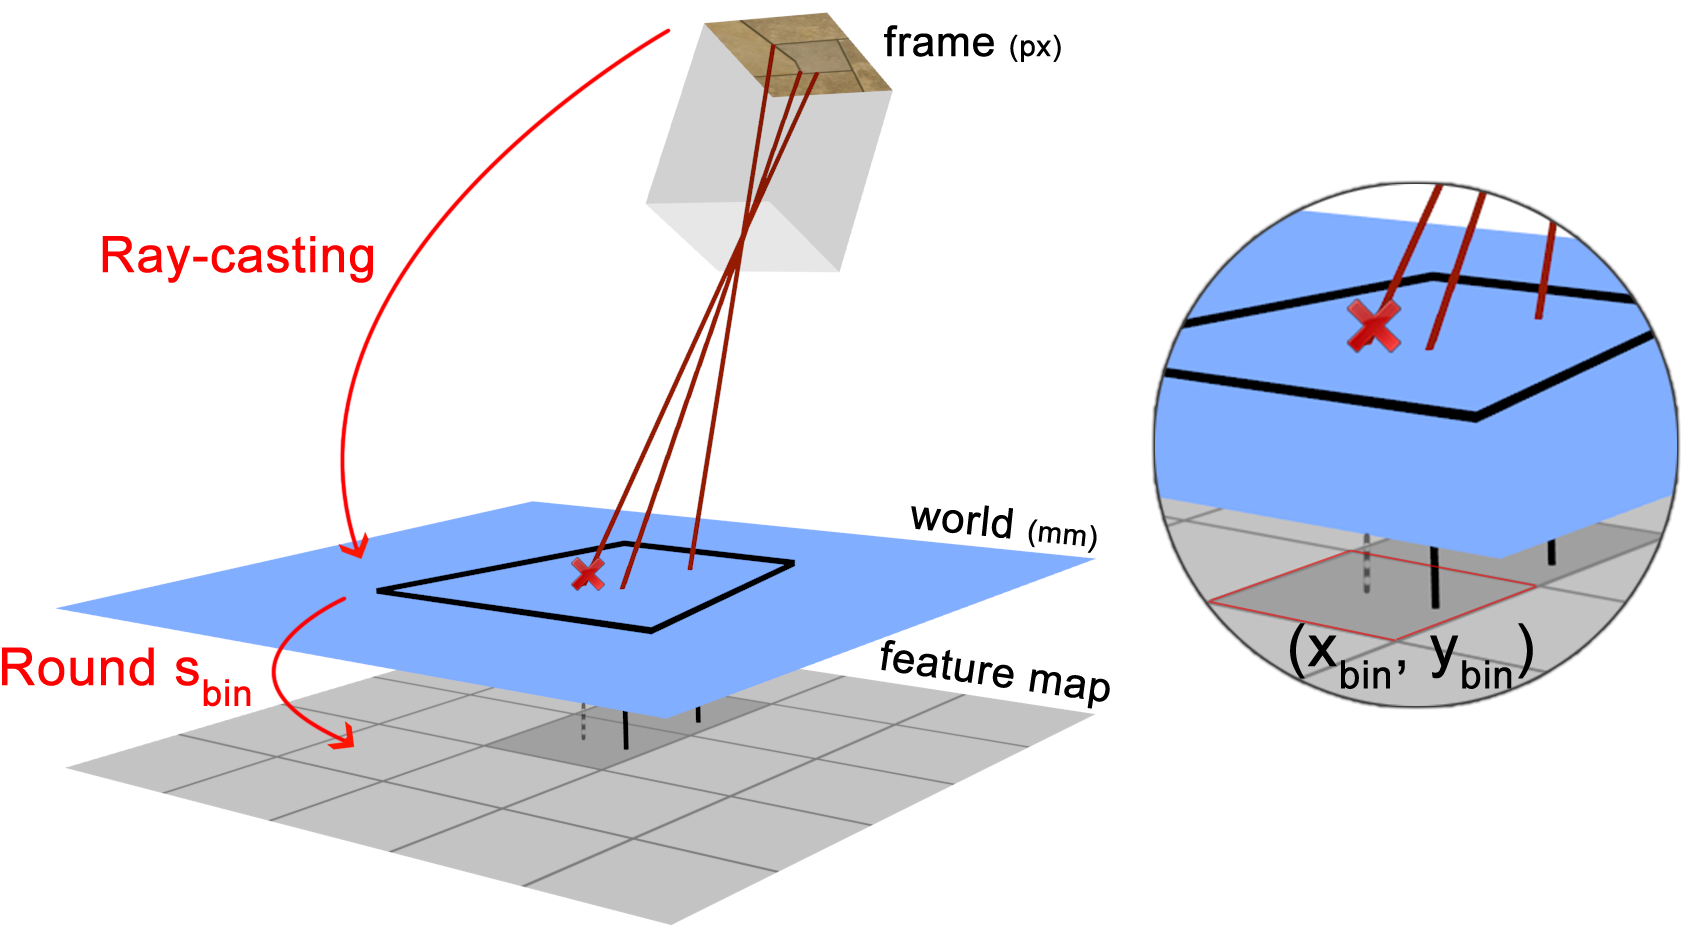
\includegraphics[width=10cm]{images/mapping3.png}
\caption{Feature map: adding visual features to a feature grid. Each feature found in the camera frame is mapped to the corresponding 2D world coordinates. The 2D world coordinates are mapped to the grid cell the feature belongs to. For each cell, only the best feature is stored.}
\label{fig:mapping3}
\end{figure}

A 2D grid with a fixed resolution of $100 \times 100mm$ per cell is used.
%which is nearly equivalent with $20 \times 20\small{px}$.
%Each grid cell corresponds to an area of $100 \times 100\small{mm}$ of the world.
From each camera frame we extract Speeded-Up Robust Features (SURF) \cite{Bay2008cviu} that are invariant with respect to rotation and scale.
% SURF features are scale- and rotation-invariant. See Bay2008cviu
Each feature is an abstract description of an "interesting" part of an image (e.g., corners).
A feature is described by a center point in image sub-pixel coordinates and a descriptor vector that consists of 64 floats.

Each feature that is detected in a camera frame is mapped to the corresponding cell of the feature map.
A feature's center point ($x_f, y_f$) is transformed to its corresponding position in 2D world coordinates ($x_w, y_w$), visible in the top of Figure \ref{fig:mapping3}.
This is done by casting a ray from the features pixel coordinates in the frame.
The method is similar to the method used for casting ray's from the frame's corners (Section \ref{sec:texture_map}).
Finally, the 2D world position ($x_w, y_w$) of each feature is transformed to the corresponding cell indices ($x_{bin}, y_{bin}$), visible in the bottom of Figure \ref{fig:mapping3}.

\begin{equation}
\left[ {
\begin{array}{c} x_{bin} \\ y_{bin} \end{array}
} \right]
=
Round(
s_{bin}
\cdot
\left[ {
\begin{array}{c} x_{w} \\ y_{w} \end{array}
} \right]
)
\end{equation}
where $s_{bin} = 0.01$.

For each cell, only the best feature (e.g. with the highest response) is kept and the other features are dropped.
%If a cell is already connected to a feature descriptor ($grid_{x,y} \neq \emptyset$), the cell is ignored.
If a cell already contains a feature descriptor ($grid_{x,y} \neq \emptyset$), the cell is ignored.

\begin{equation}
grid_{x,y} = 
\begin{cases}
\arg\max_{d \in D_{x,y}} response(d) & \mbox{if }  grid_{x,y} = \emptyset \\
grid_{x,y}   &   \mbox{else}
\end{cases} 
\end{equation}
where $D_{x,y}$ is the set of features that is mapped to cell $x_{bin} ,y_{bin}$.

%The remaining feature descriptors, including the corresponding world coordinates $x_w, y_w$, are added at the end of a descriptor matrix.
%The indices of these descriptors are written to the corresponding cell of the grid.
%This way, each cell of the grid is connected to a descriptor from the descriptors matrix.
The remaining (best) feature descriptors, including the corresponding world coordinates ($x_w, y_w$), are added to the corresponding grid cells.


\begin{comment}
\subsubsection{Processing time}

Processing a single frame and adding it to the map requires approximately $130\small{ms}$ (visual mapping: $20\small{ms}$, feature mapping: $110\small{ms}$).
The AR.Drone's framerate is fixed at 15fps, which is too high to process each single frame in realtime.
In order to achieve realtime mapping, frames that are receiving while another frame is still being process, are dropped.
However, the processing is sufficiently fast to enable seamlessly mapping.
For example, when flying at $1\small{m}$ altitude, the camera (64 degree FOV) perceives $1.24\small{m}$ floor.
The maximum horizontal speed to achieve seamlessly mapping at 15fps is 
% $(1.24 * 15 = 
$18.75\small{m/s}$, which is nearly four times the default maximum speed of the AR.Drone ($5\small{m/s}$).
With reduced framerate (7.7fps instead of 15 fps), the maximum horizontal speed is 
% $1.24 * 7.7 = 
$9.55\small{m/s}$, which is significantly faster than the AR.Drone's default maximum speed.
\end{comment}


	\section{Localization}

The feature map created in the previous section can be used for absolute position estimates, at the moment of loop-closure (when the AR.Drone is above a location where it has been before).
This allows to correct the drift that originates from the internal sensors of the AR.Drone.
The inertia measurements provide frequent position estimates.
However, the estimated position will drift over time, because the errors of the inertia measurements being accumulated.
The feature map that is created can be exploited to reduce this drift, because localization against this map provides absolute positions of the vehicle.
These absolute positions are integrated into the EKF and improve the estimated position and reduce the covariance of the state.

When a camera frame is received, SURF features are extracted.
Each feature consists of a center position in pixel coordinates ($x_f, y_f$) and a feature descriptor.
A feature's center point ($x_f, y_f$) is transformed to its corresponding position in 2D world coordinates ($x_w, y_w$), visible in the top of Figure \ref{fig:mapping3}.
This is done by casting a ray from the features pixel coordinates in the frame.
The method is similar to the method used for casting ray's from the frame's corners (Section \ref{sec:texture_map}).

%The pixel coordinates of the features are transformed to 2D world coordinates.
%The method used is already described in Section X.

The next step is matching the feature descriptors from the camera frame against the feature descriptors from the feature map.
When the feature map is quite large, this process becomes slow.
However, the estimated position of the vehicle can be used to select a subset of the feature map.
This can be done by placing a window that is centered at the vehicle's estimated position.
The covariance of the estimated position can be used to determine the size of the window.
The set of frame descriptors (query descriptors $D_q$) is matched against the map descriptors (training descriptors $D_t$).
Matching is done using a brute force matcher that uses the $L^2$ norm as similarity measure.
For each query descriptor $d_q$ from the frame, function $C(d_q)$ selects the training descriptor $d_t$ from the map that minimizes the $L^2$ norm:


\begin{equation}
C(d_q) = \arg\min_{d_t \in D_T} L2(d_q, d_t)
\end{equation}
where $D_T$ is the set of map descriptors within a window around the estimated position.
The $L2$ distance between two descriptors $a$ and $b$ is defined as:

\begin{equation}
L2(a,b) =\sqrt { \sum_{i=1}^{N} \left| a_i - b_i \right| ^2 }
\end{equation}
where $N = 64$ is the length of the SURF descriptor vector.

Each query descriptor (frame) is matched against the descriptor from the training descriptors (map) that is most similar.
Please note it is possible that multiple descriptors from the frame are matched against a single descriptor from the map.

For each match $C(d_q, d_t)$ the 2D world coordinates $(x_{w, d_q}, y_{w, d_q})$ and $(x_{w, d_t}, y_{w, d_t})$ of both descriptors are already computed.
These point pairs can be used to calculate a transformation between the query points (frame) and training (map) points.
This transformation describes the relation between the EKF estimated vehicle position (described in Section~\ref{sec:EKF}) and the position according to the feature map.

\begin{figure}[htb]
\centering
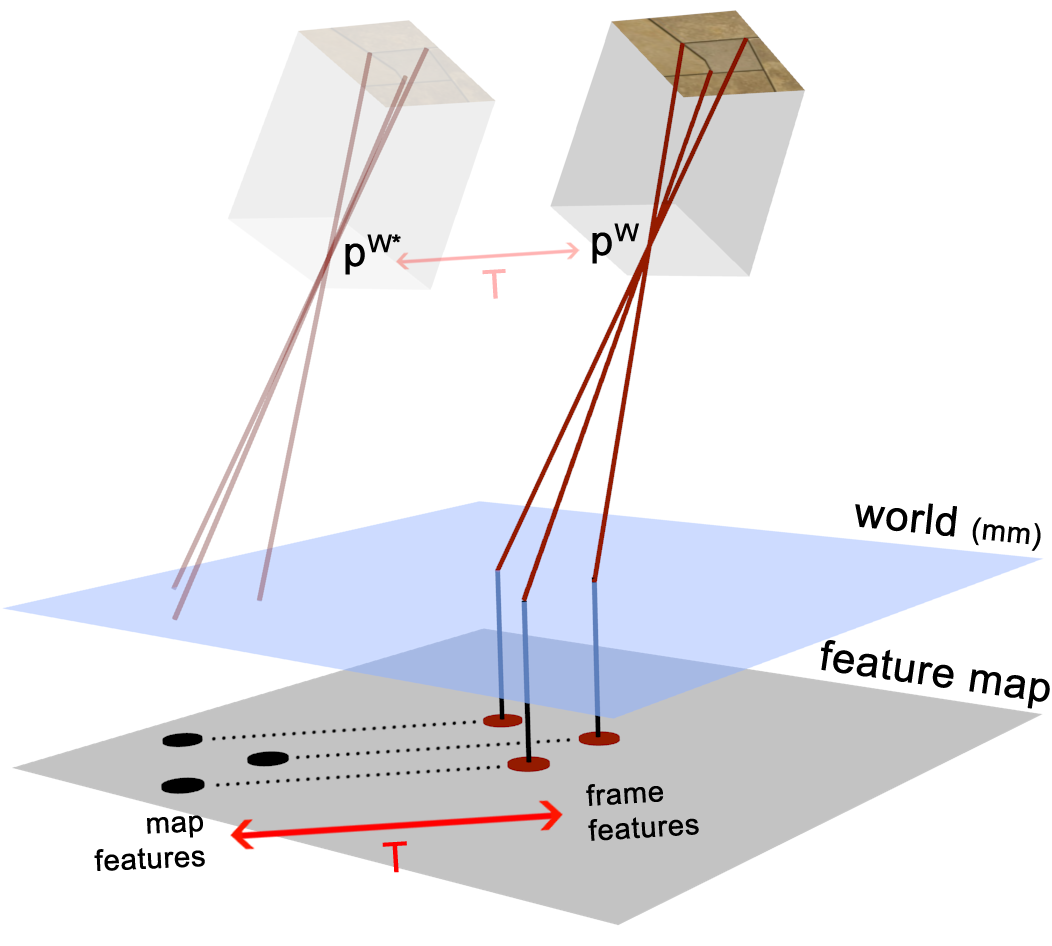
\includegraphics[width=9cm]{images/localization1.png}
\caption{Localization: features from the camera frame (red circles) are matched against the features from the feature map (black circles). All the feature points (pixels) are converted to 2D word coordinates. The translation $T$ between both feature sets is calculated and used to correct the estimated position of the AR.Drone.}
\label{fig:localization1}
\end{figure}

Different types of transformations can be used to describe the relation between the point pairs (e.g., perspective transformation or affine transformation).
However, if not all of the point pairs fit the transformation (due to outliers), the initial transformation estimate will be poor.
We use Random Sample Consensus (RANSAC) \cite{fischler1981random} to filter the set of matches in order to detect and eliminate erroneous matches (point pairs).
RANSAC tries different random subsets of corresponding point pairs.
It estimates the transformation using this subset and then computes the quality of the computed transformation by counting the number of inliers.

Since the point pairs are normalized,
%,(i.e., all pixel coordinates are transformed to 2D world coordinates),
the perspective deformation and scale differences between the point pairs (matches) are already removed.
The remaining degrees of freedom are the translation and rotation between the point pairs. 
Perspective transformation and affine transformation provide more degrees of freedom than required.
This is potentially dangerous, because an incorrect transformation may still results in a high percentage of inliers.
For example, this may happen when multiple query descriptors (frame) are matched against a single training descriptor (map).
In that case, a perspective or affine transformation is found that scales all points to a single position.
This transformation does not correspond with the actual translation and rotation, but is a valid transformation according to the RANSAC algorithm.

Instead of computing a full perspective, affine or Euclidean transformation, here only the translation in $x$ and $y$ direction is estimated. The rotation is estimated independently, as described at the end of this section.
The translation is estimated by taking a subset of 3 random point pairs.
The translation for those points is computed as follows:

\begin{comment}
$M_{train} = \begin{pmatrix}
x_{0,t,w} & y_{0,t,w}
\\
x_{1,t,w} & y_{1,t,w}
\\
x_{2,t,w} & y_{2,t,w}
\end{pmatrix}$

$M_{query} = \begin{pmatrix}
x_{0,q,w} & y_{0,q,w}
\\
x_{1,q,w} & y_{1,q,w}
\\
x_{2,q,w} & y_{2,q,w}
\end{pmatrix}$

\begin{equation}
T = (M_{train} - M_{query}) / N
\end{equation}


\begin{equation}
T =
\left[ {
\begin{array}{c}
 \frac{\sum_{i}^{N} (x_{t,w} - x_{q,w})}{N}
\\
 \frac{\sum_{i}^{N} (y_{t,w} - y_{q,w})}{N}
\end{array}
} \right]
\end{equation}


\end{comment}


\begin{equation}
T_x = \frac{\sum_{i}^{N} (x_{w, d_t, i} - x_{w, d_q, i})}{N}
\end{equation}
\begin{equation}
T_y = \frac{\sum_{i}^{N} (y_{w, d_t ,i} - y_{w, d_q, i})}{N}
\end{equation}
where $N = 3$ is the number of point pairs.

The standard deviation of translation  $T$ is defined as:

\begin{equation}
\sigma_x = \sqrt{  \sum_{i}^{N}   ((x_{w, d_t} - x_{w, d_q}) - T_x)^{2}   }
\end{equation}
\begin{equation}
\sigma_y = \sqrt{  \sum_{i}^{N}   ((y_{w, d_t} - y_{w, d_q}) - T_y)^{2}   }
\end{equation}

The confidence $c$ of translation $T$ is computed using the standard deviation:

\begin{equation}
c_{T} = 1 -   \sigma_x / \theta_{d} -  \sigma_y / \theta_{d}
\end{equation}
where $\theta_d$ = 200.

After RANSAC has performed all iterations, the translation with highest confidence $T_{best}$ is used as final translation.
A big advantage of this two degrees of freedom approach is that it is very efficient, allowing a great number of RANSAC iterations to find the optimal subset of point pairs.
If the confidence $c_{T}$ of the translation $T_{best}$ exceeds a threshold, the transformation $T$ is added to the estimated position $p^W$ to compute the corrected position $p^{W*}$. This corrected position is integrated in the EKF as measurement with low covariance.
Please note this method requires that the estimated yaw of the vehicle is close to the actual yaw.
A large difference between estimated and actual yaw results in low confidence $c_T$.
Localization on regular basis should sufficiently correct errors in the estimated yaw.

If the confidence is exceptionally high (i.e., good matches are found), the selected point pairs are used to determine the rotation between the estimated yaw and the real yaw of the vehicle. This rotation is used to correct the drift in yaw.
The rotation is computed using Kabsch algorithm \cite{Kabsch:a12999}.
This method computes the optimal rotation matrix that minimizes the RMSD (root mean squared deviation) between two paired sets of points.
Like the translation, the rotation is added to the estimated rotation to calculate the correct rotation. This rotation is directly written to the EKF state.

This localization method allows us to exploit the feature map created in Section~\ref{sec:feature_map} and get absolute position estimates which can be used to autonomously navigate the AR.Drone, as demonstrated in the next section.


		\subsection{Pose recovery approaches}
			\subsubsection{Correcting for translation}
			\subsubsection{Correcting for rotation}
	\section{Elevation mapping using an ultrasound sensor}
		\subsection{Detecting elevations}
